\section{Introduction to Languages,IDE’s,Tools and Technologies used for Implementation}
	
\subsection{Technologies used}

\subsubsection{MATLAB}
 MATLAB (matrix laboratory) is a multi-paradigm numerical computing environment. A proprietary programming language developed by MathWorks, MATLAB allows matrix manipulations, plotting of functions and data, implementation of algorithms, creation of user interfaces, and interfacing with programs written in other languages, including C, C++, Java, Fortran and Python.

Although MATLAB is intended primarily for numerical computing, an optional toolbox uses the MuPAD symbolic engine, allowing access to symbolic computing abilities. An additional package, Simulink, adds graphical multi-domain simulation and model-based design for dynamic and embedded systems.

As of 2017, MATLAB has roughly 1 million users across industry and academia. MATLAB users come from various backgrounds of engineering, science, and economics.

\begin{itemize}

\item \textbf{Setting up a project}

To setup our project, user needs to have a opertaion system along with matlab installed in it. Operting system such as windows, linux will be sufficient to perform retinal image detection.

\begin{figure}[ht]
\centering
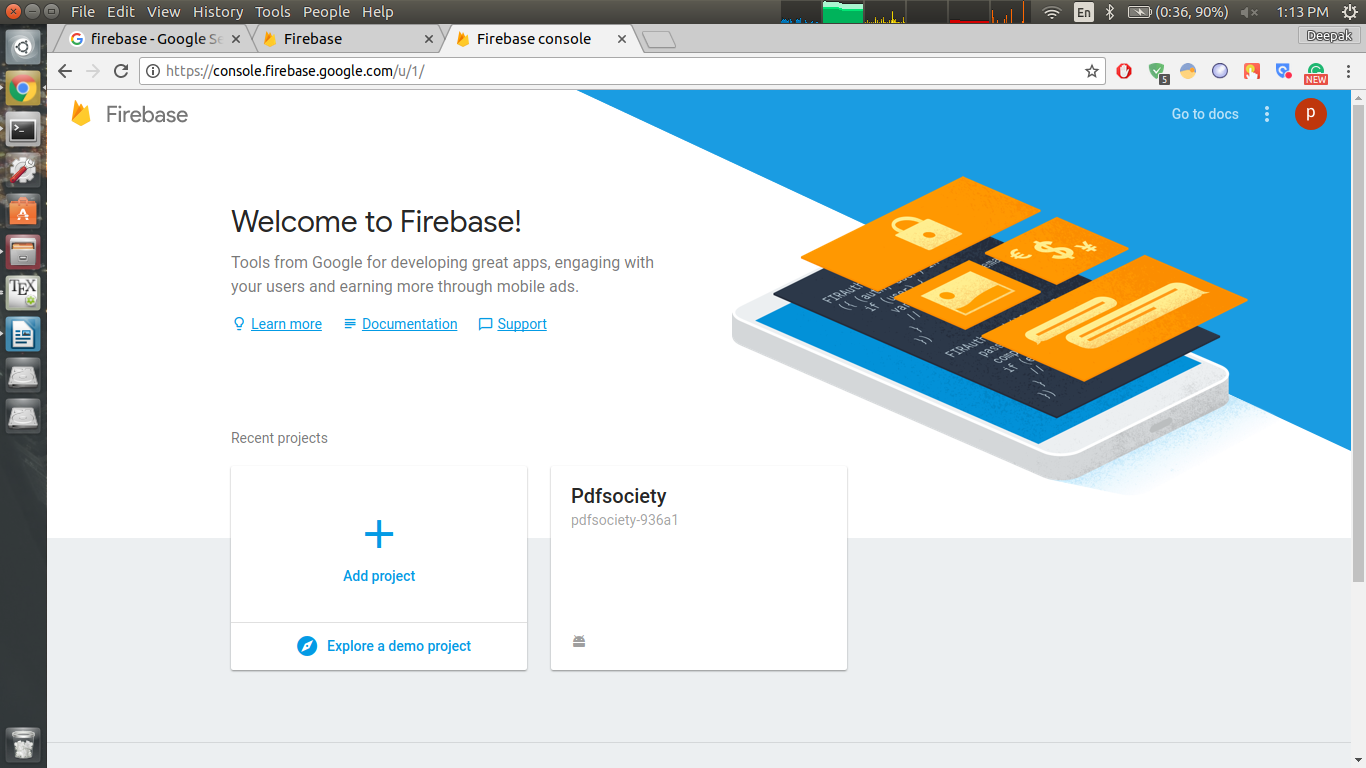
\includegraphics[scale=0.20]{images/Pdf2.png}
\caption{Firebase Console}
\end{figure}

 

\item \textbf{Firebase Products}

\begin{figure}[ht]
\centering
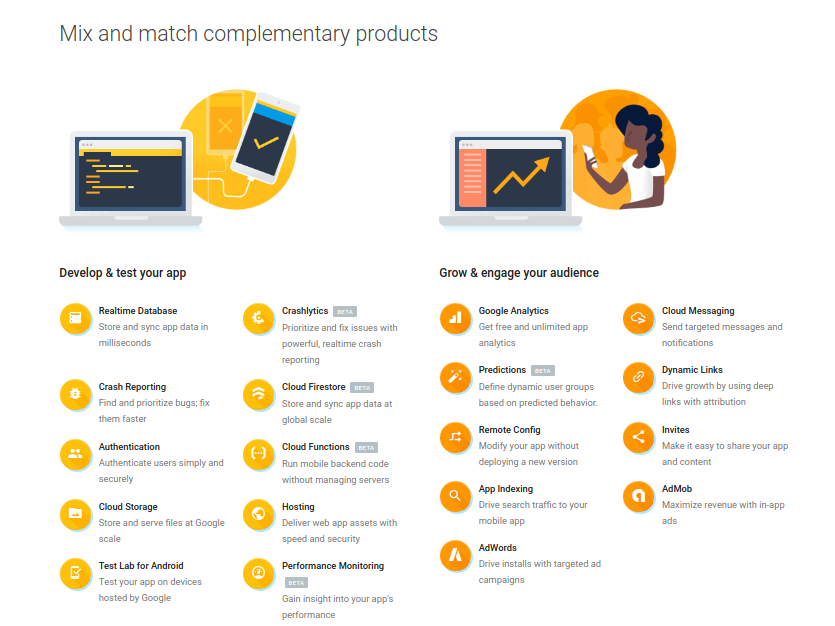
\includegraphics[scale=0.4]{images/Pdf1.png}
\caption{Firebase Products}
\end{figure}

\begin{itemize}

\item \textbf{DRIVE}

The DRIVE database has been established to enable comparative studies on segmentation of blood vessels in retinal images. The research community is invited to test their algorithms on this database and share the results with other researchers through this web site. On this page, instructions can be found on downloading the database and uploading results, and the results of various methods can be inspected. \\

The data included in this database can be used, free of charge, for research and educational purposes. Copying, redistribution, and any unauthorized commercial use is prohibited. The use of this database is restricted to those individuals or organizations that obtained the database directly from this website. Any researcher reporting results which use this database must acknowledge the DRIVE database. We request you to do so by citing this publication:

\item \textbf{Cloud Storage}

Cloud Storage is built for app developers who need to store and serve user-generated content, such as photos or videos.

Cloud Storage for Firebase is a powerful, simple, and cost-effective object storage service built for Google scale. The Firebase SDKs for Cloud Storage add Google security to file uploads and downloads for your Firebase apps, regardless of network quality. You can use our SDKs to store images, audio, video, or other user-generated content. On the server, you can use Google Cloud Storage, to access the same files.
	\end{itemize}
	\end{itemize}
	
\subsubsection{Web Technology}


Web technology is a broad term for the work involved in developing a web site for the Internet (World Wide Web) or an intranet (a private network). Web development can range from developing the simplest static single page of plain text to the most complex web-based internet applications (or just 'web apps') electronic businesses, and social network services. A more comprehensive list of tasks to which web development commonly refers, may include web engineering, web design, web content development, client liaison, client-side/server-side scripting, web server and network security configuration, and e-commerce development. Among web professionals, "web development" usually refers to the main non-design aspects of building web sites: writing markup and coding. 

\begin{figure}[ht]
\centering
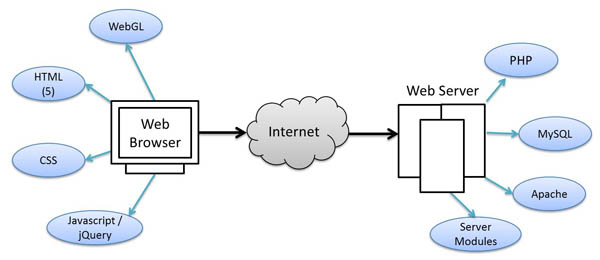
\includegraphics[scale=0.48]{images/WebTechnology.jpg}
\caption{Web Development Anatomy}
\label{fig:Anatomy}
\end{figure}

Most recently Web development has come to mean the creation of content management systems or CMS. These CMS can be made from scratch, proprietary or open source. In broad terms the CMS acts as middleware between the database and the user through the browser. A principle benefit of a CMS is that it allows non-technical people to make changes to their web site without having technical knowledge.

For larger organizations and businesses, web development teams can consist of hundreds of people (web developers) and follow standard methods like Agile methodologies while developing websites. Smaller organizations may only require a single permanent or contracting developer, or secondary assignment to related job positions such as a graphic designer or information systems technician. Web development may be a collaborative effort between departments rather than the domain of a designated department. There are three kinds of web developer specialization: front-end developer, back-end developer, and full-stack developer. Front-end developers deal with the layout and visuals of a website, while back-end developers deal with the functionality of a website. Back-end developers will program in the functions of a website that will collect data.
Since the commercialization of the web, web development has been a growing industry. The growth of this industry is being driven by businesses wishing to use their website to sell products and services to customers.[1]

There is open source software for web development like BerkeleyDB, GlassFish, LAMP (Linux, Apache, MySQL, PHP) stack and Perl/Plack. This has kept the cost of learning web development to a minimum. Another contributing factor to the growth of the industry has been the rise of easy-to-use WYSIWYG web-development software, such as Adobe Dreamweaver, BlueGriffon and Microsoft Visual Studio. Knowledge of HyperText Markup Language (HTML) or of programming languages is still required to use such software, but the basics can be learned and implemented quickly with the help of help files, technical books, internet tutorials, or face-to-face training.



\begin{itemize}

\item \textbf{Activity Lifecycle}
Activities in the system are managed as an activity stack. When a new activity
is started, it is placed on the top of the stack and becomes the running activitythe previous activity always remains below it in the stack, and will not come to
the foreground again until the new activity exits. An activity has essentially four
states:
If an activity in the foreground of the screen (at the top of the stack), it is
active or running.

If an activity has lost focus but is still visible (that is, a new non-full-sized or
transparent activity has focus on top of your activity), it is paused. A paused
activity is completely alive (it maintains all state and member information and
remains attached to the window manager), but can be killed by the system in
extreme low memory situations.


\end{itemize}

\subsection{Language used}
\subsubsection{FORTAN}

Fortran
Fortran acs cover.jpeg
The Fortran Automatic Coding System for the IBM 704 (15 October 1956), the first Programmer's Reference Manual for Fortran
Paradigm	multi-paradigm: structured, imperative (procedural, object-oriented), generic
Designed by	John Backus
Developer	John Backus and IBM
First appeared	1957; 61 years ago
Stable release	
Fortran 2008 (ISO/IEC 1539-1:2010) / 2010; 8 years ago
Typing discipline	strong, static, manifest
Filename extensions	.f, .for, .f90
Major implementations
Absoft, Cray, GFortran, G95, IBM XL Fortran, Intel, Hitachi, Lahey/Fujitsu, Numerical Algorithms Group, Open Watcom, PathScale, PGI, Silverfrost, Oracle Solaris Studio, Visual Fortran, others
Influenced by
Speedcoding
Influenced
ALGOL 58, BASIC, C, Chapel,[1] CMS-2, Fortress, PL/I, PACT I, MUMPS and Ratfor
Fortran (/ˈfɔːrtræn/; formerly FORTRAN, derived from Formula Translation[2]) is a general-purpose, imperative programming language that is especially suited to numeric computation and scientific computing. Originally developed by IBM[3] in the 1950s for scientific and engineering applications, FORTRAN came to dominate this area of programming early on and has been in continuous use for over half a century in computationally intensive areas such as numerical weather prediction, finite element analysis, computational fluid dynamics, computational physics, crystallography and computational chemistry. It is a popular language for high-performance computing[4] and is used for programs that benchmark and rank the world's fastest supercomputers.[5]

Fortran encompasses a lineage of versions, each of which evolved to add extensions to the language while usually retaining compatibility with prior versions. Successive versions have added support for structured programming and processing of character-based data (FORTRAN 77), array programming, modular programming and generic programming (Fortran 90), high performance Fortran (Fortran 95), object-oriented programming (Fortran 2003) and concurrent programming (Fortran 2008).

The characteristics and features of java are as follows :

\begin{itemize}
	\item 

Matlab is easy to understand because of its user interface. It has a very friendly user interface.  


\item The main reason is that Matlab is dynamically typed. That is, a variable can change type as it is modified.


\begin{itemize}
	\item Functional programming language
	
\item Support for objects

\end{itemize}

\item \textbf{Secure}
Matlab is Secure Language because of its many features it enables to
develop virus-free, tamper-free systems. Authentication techniques are
based on public-key encryption.

\item \textbf{Robust}

Robust Javascript was created as a strongly typed language. Data type issues
and problems are resolved at compile-time, and implicit casts of a variable
from one type to another are not allowed.

\item \textbf{Architectural Neural}
Architecture neutral It is not easy to write an application that can be used
on Windows , UNIX and a Macintosh. And its getting more complicated
with the move of windows to non Intel CPU architectures.
matlab takes a diffierent approach. 
\item \textbf{Portable}
Portable matlab code is portable. It was an important design goal of Javascript that it
be portable so that as new architectures(due to hardware, operating system,
or both)

\item \textbf{High performance}
High performance For all but the simplest or most infrequently used appli-cations,
performance is always a consideration for most applications, including
21graphics-intensive ones such as are commonly found on the world wide web,
the performance of matlab is more than adequate.



\end{itemize}

\subsection{IDE used}
\subsubsection{Matlab}

\begin{figure}[ht]
\centering

\includegraphics[scale=0.90]{images/VisualStudio.png}
\caption{Visual Studio}
\end{figure}

MATLAB (matrix laboratory) is a multi-paradigm numerical computing environment. A proprietary programming language developed by MathWorks, MATLAB allows matrix manipulations, plotting of functions and data, implementation of algorithms, creation of user interfaces, and interfacing with programs written in other languages, including C, C++, Java, Fortran and Python.\\
Although MATLAB is intended primarily for numerical computing, an optional toolbox uses the MuPAD symbolic engine, allowing access to symbolic computing abilities. An additional package, Simulink, adds graphical multi-domain simulation and model-based design for dynamic and embedded systems.

As of 2017, MATLAB has roughly 1 million users across industry and academia. MATLAB users come from various backgrounds of engineering, science, and economics





\begin{itemize}
\item \textbf{System Requirements}
Web application development on either of the following operating systems −
\vskip 0.1in

Microsoft Windows 10/8/7/Vista/2003 (32 or 64-bit)
\\Mac OS X 10.8.5 or higher, up to 10.9 (Mavericks)
\\GNOME or KDE desktop
\vskip 0.1in

\end{itemize}

\subsection{Introduction to \LaTeX}
\begin{figure}[ht]
\centering

\includegraphics[scale=0.2]{images/latex.png}
\caption{\LaTeX{} Logo}
\end{figure}
\hspace{-1.8em} \LaTeX{}, I had never heard about this term before doing this project,
but when I came to know about it's features, it is just excellent. 
\LaTeX (pronounced /ˈleɪtɛk/, /ˈleɪtɛx/, /ˈlɑːtɛx/, or /ˈlɑːtɛk/) is a 
document markup language and document preparation system for the \TeX{} 
typesetting  program. Within the typesetting system, its name is styled 
as \LaTeX.

\hspace{-1.8em} Within the typesetting system, its name is styled as \LaTeX. The term 
\LaTeX{} refers only to the language in which documents are written, 
not to the editor used to write those documents. In order to create a 
document in \LaTeX, a .tex file must be created using some form of text 
editor. While most text editors can be used to create a \LaTeX{} document, 
a number of editors have been created specifically for working with \LaTeX.\\

\noindent\LaTeX{} is most widely used by mathematicians, scientists, 
engineers, philosophers, linguists, economists and other scholars in 
academia. As a primary or intermediate format, e.g., translating DocBook 
and other XML-based formats to PDF, \LaTeX{} is used because of the 
high quality of typesetting achievable by \TeX. The typesetting system 
offers programmable desktop publishing features and extensive facilities 
for automating most aspects of typesetting and desktop publishing, 
including numbering and cross-referencing, tables and figures, 
page layout and bibliographies.\\

\noindent\LaTeX{} is intended to provide a high-level language that
accesses the power of \TeX. \LaTeX{} essentially comprises a
collection of \TeX{} macros and a program to process \LaTeX documents. 
Because the \TeX{} formatting commands are very low-level, it is usually 
much simpler for end-users to use \LaTeX{}.


\subsubsection{Typesetting}
\LaTeX{} is based on the idea that authors should be able to focus on 
the content of what they are writing without being distracted by its 
visual presentation. in preparing a \LaTeX{} document, the author 
specifies the logical structure using familiar concepts such as 
chapter, section, table, figure, etc., and lets the \LaTeX{} system 
worry about the presentation of these structures. it therefore 
encourages the separation of layout from content while still allowing 
manual typesetting adjustments where needed. 

\begin{verbatim}
\documentclass[12pt]{article}
\usepackage{amsmath}
\title{\LaTeX}
\begin{document}
  \maketitle 
  \LaTeX{} is a document preparation system 
  for the \TeX{} typesetting program.
   \par 
   $E=mc^2$
\end{document}
\end{verbatim}

\subsubsection{Installing \LaTeX{} on System}
Installation of \LaTeX{} on personal system is quite easy. As i have used \LaTeX{} on Ubuntu 13.04 so i am discussing the installation steps for Ubuntu 13.04 here:
\begin{itemize}
\item Go to terminal and type\\\\
\textit{sudo apt-get install texlive-full}
\item Your Latex will be installed on your system and you can check for manual page by typing.\\\\
\textit{man latex}\\

in terminal which gives manual for latex command.
\item To do very next step now one should stick this to mind that the document which one is going to produce is written in any type of editor whether it may be your most common usable editor Gedit or you can use vim by installing first vim into your system using command.\\\\
\textit{sudo apt-get install vim}
\item After you have written your document it is to be embedded with some set of commands that Latex uses so as to give a structure to your document. Note that whenever you wish your document to be looked into some other style just change these set of commands.
\item When you have done all these things save your piece of code with .tex format say test.tex. Go to terminal and type\\\\
\textit{latex path of the file test.tex Or pdflatex path of the file test.tex\\ eg: pdflatex test.tex}\\
for producing pdf file simultaneously.\\
After compiling it type command\\\\
\textit{evince filename.pdf\\ eg: evince test.pdf}\\
To see output pdf file. 
\end{itemize}
\subsubsection{Pdfscreen \LaTeX{}}
There are some packages that can help to have unified document using \LaTeX{}. Example of such a package is pdfscreen that let the user view it’s document in two forms-print and screen. Print for hard copy and screen for viewing your document on screen. Download this package from www.ctan.org/tex-archive/macros/latex/contrib/pdfscreen/.\\
Then install it using above mention method.\\

\noindent To test it the test code is given below:-\\
Just changing print to screen gives an entirely different view. But for working of pdfscreen another package required are comment and fancybox.\\

\noindent The fancybox package provides several different styles of boxes for framing and rotating content in your document. Fancybox provides commands that produce square-cornered boxes with single or double lines, boxes with shadows, and round-cornered boxes with normal or bold lines. You can box mathematics, floats, center, flushleft, and flushright, lists, and pages.\\
 	
\noindent Whereas comments package selectively include/excludes portions of text. The comment package allows you to declare areas of a document to be included or excluded. One need to make these declarations in the preamble of your file. The package uses a method for exclusion that is pretty robust, and can cope with ill-formed bunches of text.\\

\noindent So these extra packages needed to be installed on system for the proper working of pdfscreen package.


	\section{Coding standards of Language used 
}

\subsection{Coding standards for Javascript }
\begin{itemize}

\item Preprocessor Where the use of a language preprocessor is required, it will be the C preprocessor (cpp). cpp is available on any UNIX platform, and many Fortran compilers have the ability to run cpp automatically as part of the compilation process. All tokens will be uppercase to distinguish them from Fortran code, which will be in lower case.

\item F90 Standard CCM4 will adhere to the Fortran 90 language standard. The purpose is to enhance portability, and to allow use of the many desirable new features of the language. If a situation arises in which there is good reason to violate this rule and include Fortran code which is not compliant with the f90 standard, an alternate set of f90-compliant code must be provided. This is normally done through use of a C-preprocessor ifdef construct.
\item Lines should usually be no longer than 80 characters, and should not exceed 100 (counting tabs as 4 spaces). This is a “soft” rule, but long lines generally indicate unreadable or disorganized code.
\item Loops Loops should be structured with the do-end do construct as opposed to numbered loops.
\item Unary special-character operators (e.g., ++, --) must not have space next to their operand.
\item Any, and; must not have preceding space.
\item Any; used as a statement terminator must be at the end of the line.
\item Any: after a property name in an object definition must not have preceding space.
\item The? and: in a ternary conditional must have space on both sides.
\item No filler spaces in empty constructs (e.g., {}, [], fn ()).
.


\end{itemize}

	\section{GANTT chart
	}
	\begin{figure}[ht]
\centering
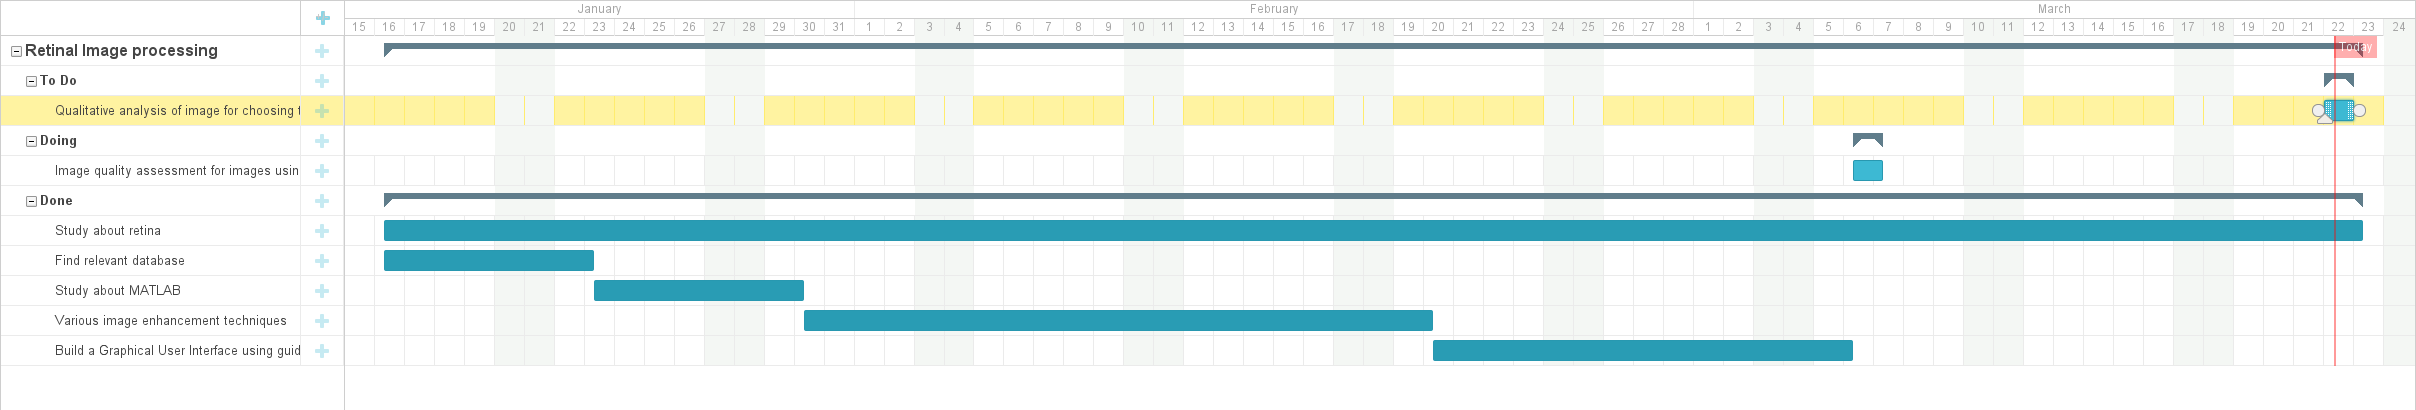
\includegraphics[scale=0.20]{images/GantChart.png}
\caption{\LaTeX{} Ghant chart}
\end{figure}
	
	\section{Testing Techniques and Test Plans
}
\subsection{Functionality Testing}
Test for – all the links in desktop application, 
submitting or getting information from user, cookie testing.

\subsection{Usability testing}
Web site should be easy to use. Instructions should be provided clearly. Check if the provided
instructions are correct meaning whether they satisfy the purpose. Main menu should be
provided on each page. It should be consistent.

\subsection{Interface Testing}
The main interfaces are:
\\ i. Web server and application server interface
\\ ii. Application server and database server interface
Check if all the interactions between these servers are executed properly. Errors are handled
properly. If database or web server returns any error message for any query by application
server, then application server should catch and display these error messages appropriately to
users. Check what happens if user interrupts any transaction in-between? Check what happens
if connection to web server is reset in between?
\subsection{Compatibility Testing}
Compatibility of your web site is very important testing aspect. See which compatibility test is
to be executed:
\\i. Browser compatibility
\\ii. Operating system compatibility
\\iii. Mobile browsing
\\iv. Printing options
\subsection{Performance Testing}
Web application should sustain to heavy load. Web performance testing should include:
\\i. Web Load Testing
\\ii. Web Stress Testing

\subsection{Security Testing}
\begin{itemize}


\item Test by pasting internal URL directly into browser address bar without login.
Internal pages should not open.
\item If you are logged in using username and password and browsing internal pages,
then try changing URL options directly, i.e., If you are checking some publisher site
statistics with publisher site ID= 123. Try directly changing the URL site ID parameter
to different site ID which is not related to logged in user. Access should be denied for
this user to view others stats.
\item Try some invalid inputs in input fields like login username, password, input text
boxes. Check the system reaction on all invalid inputs.
iv. Web directories or files should not be accessible directly unless given download
option.
\end{itemize}

